\chapter{Proof of Concept}
\label{ch:proof-of-concept}
De Proof of Concept bestaat uit een vergelijkend experiment tussen twee open source serverless (FaaS) frameworks, namelijk Fission en OpenFaaS. In dit onderdeel worden de twee frameworks opgezet op een Kubernetes cluster die bestaat uit één node. Beide frameworks worden opgezet op een MacBook Pro waarop Minikube draait. Minikube is een ''Out-of-the-box'' Kubernetes cluster. Er wordt gekozen om gebruik te maken van Minikube omdat op deze manier beide frameworks op identiek dezelfde hardware draaien. Daarnaast biedt Minikube dezelfde functionaliteiten als een volledige Kubernetes cluster die elders is opgezet. Dit hoofdstuk is opgedeeld in twee grote onderdelen waarbinnen telkens secties met dezelfde stappen voor elk framework terug te vinden zijn. Daarnaast is er ook een sectie in dit hoofdstuk terug te vinden waarin de demofunctie, die serverless gedraaid zal worden op de frameworks, wordt voorgesteld. De demo bestaat uit het deployen van een Python functie die de functionaliteit van beide frameworks demonstreert, ook wordt de uitvoeringstijd van de functie van request tot response gemeten. Later wordt er in dit onderzoek een vergelijking tussen Fission en OpenFaaS gemaakt waarbij onder meer gekeken zal worden naar het verschil in executietijd tussen de geschreven functie, de gebruiksvriendelijkheid en overige vooropgestelde requirements. Deze Proof of Concept moet meer inzicht geven in beide frameworks en geeft een duidelijk beeld van wat deze precies inhouden. Merk op dat de opstelling van deze PoC alleen een demo van beide frameworks geeft en dus niet geschikt is voor productie. Indien dit in productie wordt overgenomen dan dienen er enkele aanvullende veiligheidsmaatregelen getroffen te worden maar daar wordt in dit onderzoek niet verder op ingegaan.
\\\\
\section{Voorbereiding omgeving}
\label{sec:voorbereiding-omgeving}
\subsection{Onderliggende hardware}
\label{sec:specificaties}
Het experiment zal worden uitgevoerd op een MacBook Pro, model 2018 met volgende specificaties:
\begin{itemize}
    \item Processor: 2,2 GHz Intel Core i7.
    \item Memory: 16 GB 2400 MHz DDR4.
    \item Graphics: Radeon Pro 555X 4 GB en Intel UHD Graphics 630 1536 MB.
    \item Opslag: 256 GB SSD.
\end{itemize}

\subsection{Packet manager}
In de opstelling is het zinvol gebruik te maken van Homebrew\footnote{https://brew.sh/}, dit is een packetmanager ontwikkeld voor macOS. Homebrew zorgt ervoor dat softwarepakketten kunnen worden gedownload uit bestaande repositories. In de verdere uitwerking van dit onderzoek wordt Homebrew eveneens gebruikt voor het installeren van software.
\\\\
Homebrew kan worden geïnstalleerd door volgend commando in de Terminal uit te voeren: 
\begin{lstlisting}[language=bash]
$ /usr/bin/ruby -e "$(curl -fsSL 
https://raw.githubusercontent.com/Homebrew/install/master/install)"
\end{lstlisting}

\subsection{Softwarepakketten}
\label{sec:software}
Alvorens de frameworks kunnen worden opgezet moeten er enkele softwarepakketten aanwezig zijn. Enerzijds is Docker nodig als container engine, anderzijds Kubernetes als container platform. Daarnaast is er ook een hypervisor nodig die het draaien van een Minikube cluster mogelijk maakt. In dit onderzoek wordt gebruik gemaakt van VirtualBox\footnote{https://www.virtualbox.org/} als hypervisor, deze is open source en gratis. De softwarepakketten kunnen als volgt geïnstalleerd worden met Homebrew:        
\begin{lstlisting}[language=bash]
$ brew tap caskroom/cask
$ brew cask install virtualbox
$ brew cask install docker
$ brew cask install minikube
$ brew install kubernetes-cli
\end{lstlisting}

\subsection{Softwareversies gebruikt tijdens Proof of Concept}
\begin{itemize}
    \item VirtualBox: 6.0.4 
    \item Docker engine: 18.09.2, build 6247962
    \item Minikube: v1.0.0
    \item Kubectl client: v1.14.1
    \item Kubectl server: v1.14.0
\end{itemize}

\subsection{Configuratie Minikube}
\label{sec:configuratie-minikube}
Vooraleer de frameworks kunnen geïnstalleerd worden, wordt er een lokale Kubernetes cluster die bestaat uit één node opgezet met Minikube. Een Minikube cluster biedt dezelfde functionaliteiten als een productieomgeving waarop een Kubernetes cluster is geïnstalleerd. Er wordt gebruik gemaakt van Kubernetes als container orkestratie platform. Een orkestrator is een tool die instaat voor het management van containers en microservice applicaties. Kubernetes zorgt ervoor dat applicaties schaalbaar kunnen worden opgezet, staat in voor het volledige beheer van de containers en voorziet ''High-availability''.
In sectie \ref{sec:software} werden de benodigde softwarepakketten reeds geïnstalleerd. Indien alle stappen succesvol werden doorlopen dan kan de Minikube cluster probleemloos worden gestart volgens de stappen in onderstaand codevoorbeeld. De Minikube cluster wordt gestart met aangepaste specificaties, zijnde: vier CPUs, 8192MB geheugen en 20000MB opslag. Na de installatie wordt eerst de status van de cluster nagegaan om te kijken of alles draait zoals gevraagd. Vervolgens wordt metrics-server ingeschakeld voor het verzamelen van metrics.

\begin{lstlisting}[language=bash]
$ minikube start --cpus 4 --memory 8192
$ minikube status
host: Running
kubelet: Running
apiserver: Running
kubectl: Correctly Configured: pointing to
minikube-vm at 192.168.99.107
$ minikube addons enable metrics-server
\end{lstlisting}

\section{Python demofunctie}
\label{sec:python-demofunctie}
De werking van beide frameworks zal worden gedemonstreerd met een zelfgeschreven Python functie. De demofunctie maakt het mogelijk om via een HTTP GET request waaraan een string wordt meegegeven, de string weg te schrijven naar een Google spreadsheet bestand. Wanneer de functie wordt aangeroepen zonder een toegevoegde string dan wordt er een GET request verstuurd naar de API die via de spreadsheet een lijst teruggeeft van weggeschreven woorden uit een vastgelegde kolom. Om gebruik te kunnen maken van Google spreadsheets moet er een Google project worden aangemaakt via de Google API, deze stappen staan verder beschreven. De functie heeft op beide frameworks dezelfde functionaliteit maar de code zal echter aangepast worden aan het framework waarop de functie draait. Beide frameworks verwachten een bepaalde vorm hoe functies geschreven worden. In sectie \ref{sec:demofunctie} is de code terug te vinden voor het uitvoeren van de functie lokaal en dus niet via een FaaS framework. De code werd lokaal geschreven en getest alvorens deze werd aangepast aan de frameworks. De code in sectie \ref{sec:demofunctie} werd gebruikt als uitgangspunt voor het omvormen naar functies die voldoen aan de specifieke vereisten van beide frameworks.

\subsection{Google API}
De Python functie schrijft een string weg naar een bestand op Google spreadsheets, als deze wordt meegegeven, zo niet haalt de functie alle strings op die weggeschreven werden naar een kolom. Om gebruik te maken van een spreadsheet bestand moet eerst de API worden geconfigureerd. Daarnaast moeten ook de credentials op de demo machine worden geconfigureerd. Het Google project wordt opgezet zodat de functie data kan wegschrijven naar de spreadsheet, in sectie \ref{sec:google-api} is een gedetailleerd stappenplan terug te vinden voor het instellen van de Google API in combinatie met Google spreadsheets. Om gebruik te maken van Google API features moeten oauth2client, gspread en google-api-python-client geïnstalleerd worden. De drie packages die nodig zijn voor de uitvoer van de functie worden gebundeld in een tekstbestand ''requirements.txt''. Het bestand met requirements kan vervolgens door ''pip'' worden gebruikt voor de installatie van de softwarepakketten en is terug te vinden als bijlage \ref{sec:requirements.txt}.

\newpage
\subsection{Code demofunctie}
\label{sec:demofunctie}
\begin{lstlisting}[language=python]
import gspread
import sys
from oauth2client.service_account import ServiceAccountCredentials
# Check if a string is provided when calling the function.
if len(sys.argv) > 1:
    req = str(sys.argv[1])
else:
    req =""

def next_available_row(worksheet):
    str_list = filter(None, worksheet.col_values(1))
    return str(len(str_list)+1)

def is_empty_string(string):
    if len(string) == 0:
        return True
    else:
        return False

def get_values(worksheet):
    cell_range = 'A1:A'+ next_available_row(worksheet)
    all_cells = worksheet.range(cell_range)
    return all_cells

def handle(req):   
    # Initialize variables for Google API
    scope = ['https://spreadsheets.google.com/feeds',
    'https://www.googleapis.com/auth/drive']
    credentials = ServiceAccountCredentials
    .from_json_keyfile_name('credentials-serverless.json', scope)
    client = gspread.authorize(credentials)
    worksheet = client.open("executietijd-demofunctie").sheet1
    next_row = next_available_row(worksheet)

    if is_empty_string(req):
        string_list = []
        for cell in get_values(worksheet):
            string_list.append(cell.value)
        print str(string_list)
    else:
        worksheet.update_acell("A{}".format(next_row), req)
        print "This function wrote '",req,"' to Google Spreadsheets!"

if __name__ == "__main__":
handle(req)
\end{lstlisting}

\newpage
\section{OpenFaaS}
OpenFaaS is het eerste framework dat onder de loep wordt genomen. Het experiment wordt opgezet op een MacBook Pro die voldoet aan specificaties uit sectie \ref{sec:specificaties} en beschikt over de benodigde softwarepakketten zoals vermeld in sectie \ref{sec:software}. De stappen die doorlopen worden in het opzetten en uitvoeren van het experiment zijn steeds duidelijk gedocumenteerd en staan chronologisch gerangschikt. De installatieprocedure is eenvoudig te volgen en is reproduceerbaar aan de hand van de gedocumenteerde stappen en bijhorende scripts.

\subsection{Installatie OpenFaaS}
Indien de installatie van Minikube uit voorgaande sectie succesvol verlopen is, dan kan OpenFaaS worden geïnstalleerd. De installatie van OpenFaaS bestaat uit enkele stappen die werden omgevormd tot een shell script. Het is mogelijk dit script vanuit de Terminal uit te voeren, vervolgens start de installatie van OpenFaaS. De volledige installatie van het framework is geautomatiseerd en reproduceerbaar. Het script in bijlage \ref{sec:installatie-openfaas} onder de naam Installatiescript OpenFaaS bevat alle installatiestappen met uitleg over wat er gebeurt. De installatie is gebaseerd op een blogpost van \textcite{Ellis2017}, de founder van OpenFaaS. In de documentatie van OpenFaaS\footnote{https://docs.openfaas.com/} wordt eveneens naar deze blogpost gerefereerd als installatiehandleiding. Na de uitvoering van het script is OpenFaaS geïnstalleerd bovenop de Minikube cluster. Het installatiescript schrijft enkele omgevingsvariabelen weg naar een bestand genaamd ''artifacts.txt'', dit is terug te vinden in dezelfde directory vanwaar het installatiescript werd uitgevoerd. Er werd eerder gerefereerd naar het OpenFaaS installatiescript, dit werd eveneens in een script opgenomen dat beide frameworks in één keer installeert. Het installatiescript voor de volledige omgeving is terug te vinden in bijlage \ref{sec:installatie-frameworks}. Volgende stappen demonstreren hoe OpenFaaS kan worden geïnstalleerd. Na succesvolle afloop is OpenFaaS geïnstalleerd op de Minikube cluster.

\begin{lstlisting}
# Clone de repository van dit onderzoek.
$ git clone git@github.com:LennertMertens/BAP.git
$ cd BAP/broncode/installatie
# Indien u enkel OpenFaaS wenst te installeren voer dan volgende uit:
$ source openfaas-install.sh

# Als u alle frameworks wilt installeren op Minikube:
$ source install.sh
\end{lstlisting}

\subsection{Deployment nieuwe demofunctie}
Het OpenFaaS framework wordt getest aan de hand van een Python functie die reeds beschreven is in sectie \ref{sec:python-demofunctie}. De functie wordt gedeployed met de faas-cli tool. De code die werd geschreven, werd eveneens aangepast zodanig dat er gebruik kan worden gemaakt van Kubernetes secrets\footnote{https://docs.openfaas.com/reference/secrets/} voor het beheer van credentials die nodig zijn voor de Google API. Het deployen van een functie is slechts mogelijk wanneer alle voorgaande stappen succesvol werden uitgevoerd. Het deployen van de functie is onderverdeeld in verschillende stappen die hieronder uitgebreid worden beschreven. 

\subsubsection{1. Aanmelden via faas-cli}
Indien eerder nog niet werd ingelogd via de faas-cli dan moet dit gebeuren voor verder te gaan. Met behulp van volgend commando kan worden ingelogd, indien dit vanuit dezelfde shell als diegene waarin het installatiescript werd uitgevoerd, gebeurt. Als de omgevingsvariabelen niet ingesteld zijn, dan kunnen deze worden aangepast naar het IP adres en wachtwoord van het Tiller service account.
\begin{lstlisting}[language=bash]
$ faas-cli login -g $OPENFAAS_URL -u admin -p $PASSWORD
\end{lstlisting}

\subsubsection{2. Aanmaken Kubernetes secret}
Eerder werd er een credential account aangemaakt via Google Cloud API. De credentials die bij het aangemaakte account horen werden opgeslagen op een lokale locatie, deze credentials worden nu in een Kubernetes secret gestopt. OpenFaaS kan secrets uitlezen en deze gebruiken in functies, dit zorgt voor extra security, zo hoeven de credentials niet aanwezig te zijn in de Docker image van de functie.

\begin{lstlisting}[language=bash]
$ kubectl create secret generic secret-api-credentials \
--from-file=secret-api-credentials=credentials-serverless.json \
--namespace openfaas-fn
\end{lstlisting}

\subsubsection{3. Deploy functie}
De eerste keer dat de gebruiker een functie wil deployen, moeten er enkele stappen worden genomen: de functie moet worden geschreven, een YAML bestand met parameters specifiek voor deployment moet worden gemaakt en de gebruiker moet inloggen op Docker Hub voor het publiceren van Docker images. Als een gebruiker een functie maakt, dan wordt deze op Docker Hub geplaatst, vandaar het belang dat de gebruiker inlogt. Standaard zal een functie die wordt gedeployed een container opzetten die voortdurend draait (standaard instelling), hierdoor kan er steeds snel op een request worden gereageerd en wordt cold-start vermeden. Volgende stappen worden ondernomen wanneer de demofunctie voor het eerst wordt gedeployed.

\begin{lstlisting}[language=bash]
# 1. Login op Docker Hub.
$ docker login

# 2. Maak een nieuwe functie.
$ mkdir demo-functie; cd demo-functie

# serverless-demo is de naam die de functie zal krijgen,
# prefix is de gebruikersnaam op Docker Hub.
$ faas-cli new --lang python serverless-demo --prefix="lennertmertens"

# De inhoud van de map ziet eruit als volgt na uitvoer 
# van vorig commando.
$ ls
serverless-demo     serverless-demo.yml    template

# Vul de handler.py en requirements.txt bestanden in de folder 
# serverless-demo aan naar eigen wensen en schrijf de functie
# De inhoud van de bestanden wordt onder de code weergegeven.

# 3. Build de functie die werd geschreven.
$ faas-cli build -f serverless-demo.yml

# 4. Push de Docker image van de functie naar Docker Hub.
$ faas-cli push -f serverless-demo.yml

# 5. Deploy de functie op het OpenFaaS framework.
$ faas-cli deploy -f serverless-demo.yml
\end{lstlisting}

De bestanden voor het maken en deployen van de functie zien er als volgt uit.

\subsubsection{serverless-demo.yml}
Aan de hand van dit bestand wordt de functie gedeployed. Dit bestand is een template waaraan enkele zaken zijn toegevoegd die specifiek zijn voor de demo-omgeving die werd opgezet. In bijlage \ref{sec:serverless-demo.yml} is de inhoud van dit bestand terug te vinden. De gateway is de URL van de OpenFaaS omgeving. De image is de Docker image die wordt gebruikt voor het deployen van de functie op het framework. De ''secrets'' optie moet eveneens worden toegevoegd als er gebruik wordt gemaakt van een Kubernetes secret. Op die manier kan de functie de inhoud ervan opvragen.

\subsubsection{severless-demo/handler.py}
Onder de map serverless-demo is het handler.py bestand terug te vinden, dit is een Python script dat de functionaliteit bevat. In bijlage \ref{sec:demofunctie-openfaas} is de code te zien die specifiek voor deze opstelling wordt gebruikt. De oorspronkelijke code werd omgevormd zodanig dat deze voldoet aan de vereisten van OpenFaaS, zo verwacht het OpenFaaS framework dat functies gebruikmaken van een ''handle'' methode die wordt opgesteld gebaseerd op een template die wordt aangeboden bij het maken van een nieuwe functie.

\subsubsection{serverless-demo/requirements.txt}
Onder de serverless-demo map is ook een requirements.txt bestand terug te vinden. Het bestand bevat de dependenties waar het Python script afhankelijk van is, dit zijn packages nodig om de functie uit te voeren. De packages  nodig voor het uitvoeren van de demofunctie zijn opgelijst in bijlage \ref{sec:requirements.txt}.

\subsection{Deployment bestaande functie}
Wanneer gebruikers reeds eerder een functie op OpenFaaS hebben gemaakt die werd gepusht naar een Docker Hub repository, dan volstaat het om enkel een template file te gebruiken zoals \ref{sec:serverless-demo.yml}. De functie wordt vanaf een bestaande image gedeployed, dus het is niet meer nodig deze image opnieuw te builden. Images in Docker registries bieden de mogelijkheden dat ze eender waar kunnen worden gebruikt door iedereen of door een afgeschermde groep mensen. Het voordeel van serverless functies is dat er per functie een container wordt gebuild die alle dependenties en runtime voor een specifiek stuk code bevat. Ongeacht van de onderliggende setup kan deze functie werken wanneer ze op een OpenFaaS framework wordt gedeployed.

\begin{lstlisting}[language=bash]
# Deploy bestaande functie op het OpenFaaS framework.
$ faas-cli template pull
$ faas-cli deploy -f serverless-demo.yml
\end{lstlisting}

\subsection{Uitvoeren demofunctie}
\label{sec:openfaas-uitvoeren-functie}
De demofunctie reageert wanneer er een HTTP GET request wordt ontvangen, deze actie kan worden getriggerd op verschillende manieren. Via de UI is het mogelijk de functie aan te roepen door deze te selecteren, eventueel een ''body'' mee te geven en dan op de knop ''invoke'' te klikken. Anderzijds, en dit wordt toegepast in dit onderzoek, kan er gebruik worden gemaakt van ''curl''. Curl verstuurt een HTTP request naar de opgegeven URL. Wanneer de optie -d wordt meegegeven met het curl commando dan wordt de string die wordt meegegeven eveneens weggeschreven naar het Google spreadsheets bestand.

\begin{lstlisting}[language=bash]
# Request voor opvragen van lijst.
$ curl -X GET http://$OPENFAAS_URL/function/serverless-demo
# Request voor wegschrijven van een string.
$ curl -X GET -d 'string om weg te schrijven' 
http://$OPENFAAS_URL/function/serverless-demo
\end{lstlisting}

\subsection{Gebruik OpenFaaS}
\subsubsection{Command line tools}
Faas-cli is de command line tool die beheer van OpenFaaS voorziet aan de hand van de console. Vooraleer van start te kunnen gaan moet de gebruiker inloggen via de Terminal door volgend commando in te voeren. Het wachtwoord werd tijdens de installatie in de Terminal weggeschreven, net zoals het IP adres waarop OpenFaaS draait. Daarnaast beschikt de shell ook over omgevingsvariabelen met het wachtwoord en de URL voor OpenFaaS. De command line tools voorzien meer functionaliteiten dan de UI. Het is mogelijk om functies te deployen via de CLI, de omgeving te beheren, confidentiële sleutels en wachtwoorden te beheren.
\begin{lstlisting}[language=bash]
$ faas-cli login -g $OPENFAAS_URL -u admin -p $PASSWORD
\end{lstlisting}

\subsubsection{User Interface}
Na de installatie is het mogelijk naar de OpenFaaS UI te surfen via het IP adres van de Minikube cluster gevolgd door poortnummer 31112.
De eerste keer dient er aangemeld te worden met gebruiker ''admin'' (Deze gebruiker wordt aangemaakt in het installatiescript) en het wachtwoord dat in de Terminal werd weergegeven door het installatiescript. Na het aanmelden is de interface zoals in figuur \ref{fig:openfaas-ui} te zien. De UI ziet er vrij sober maar heel intuïtief uit, er is eveneens een mogelijkheid om een nieuwe functie te deployen via de ''Deploy New Function'' knop. Wanneer gebruikers kiezen een nieuwe functie te deployen dan kunnen ze enerzijds kiezen voor een community functie, dit zijn reeds bestaande functies die op het OpenFaaS framework kunnen gedraaid worden. Anderzijds kunnen gebruikers ook zelfgeschreven functies deployen aan de hand van deze interface. In dit onderzoek worden functies gedeployed via de command line met het faas-cli commando. Deployments van functies via de command line bieden een betere reproduceerbaarheid en is vaak sneller en makkelijker te reproduceren. Er wordt ook bewust gekozen voor de command line tools omdat niet alle serverless frameworks over een UI beschikken. De interface is een leuke nice-to-have feature en is makkelijk in gebruik voor mensen die aan de slag willen met serverless. De UI wordt eveneens standaard meegeïnstalleerd met OpenFaaS.
\begin{figure}
    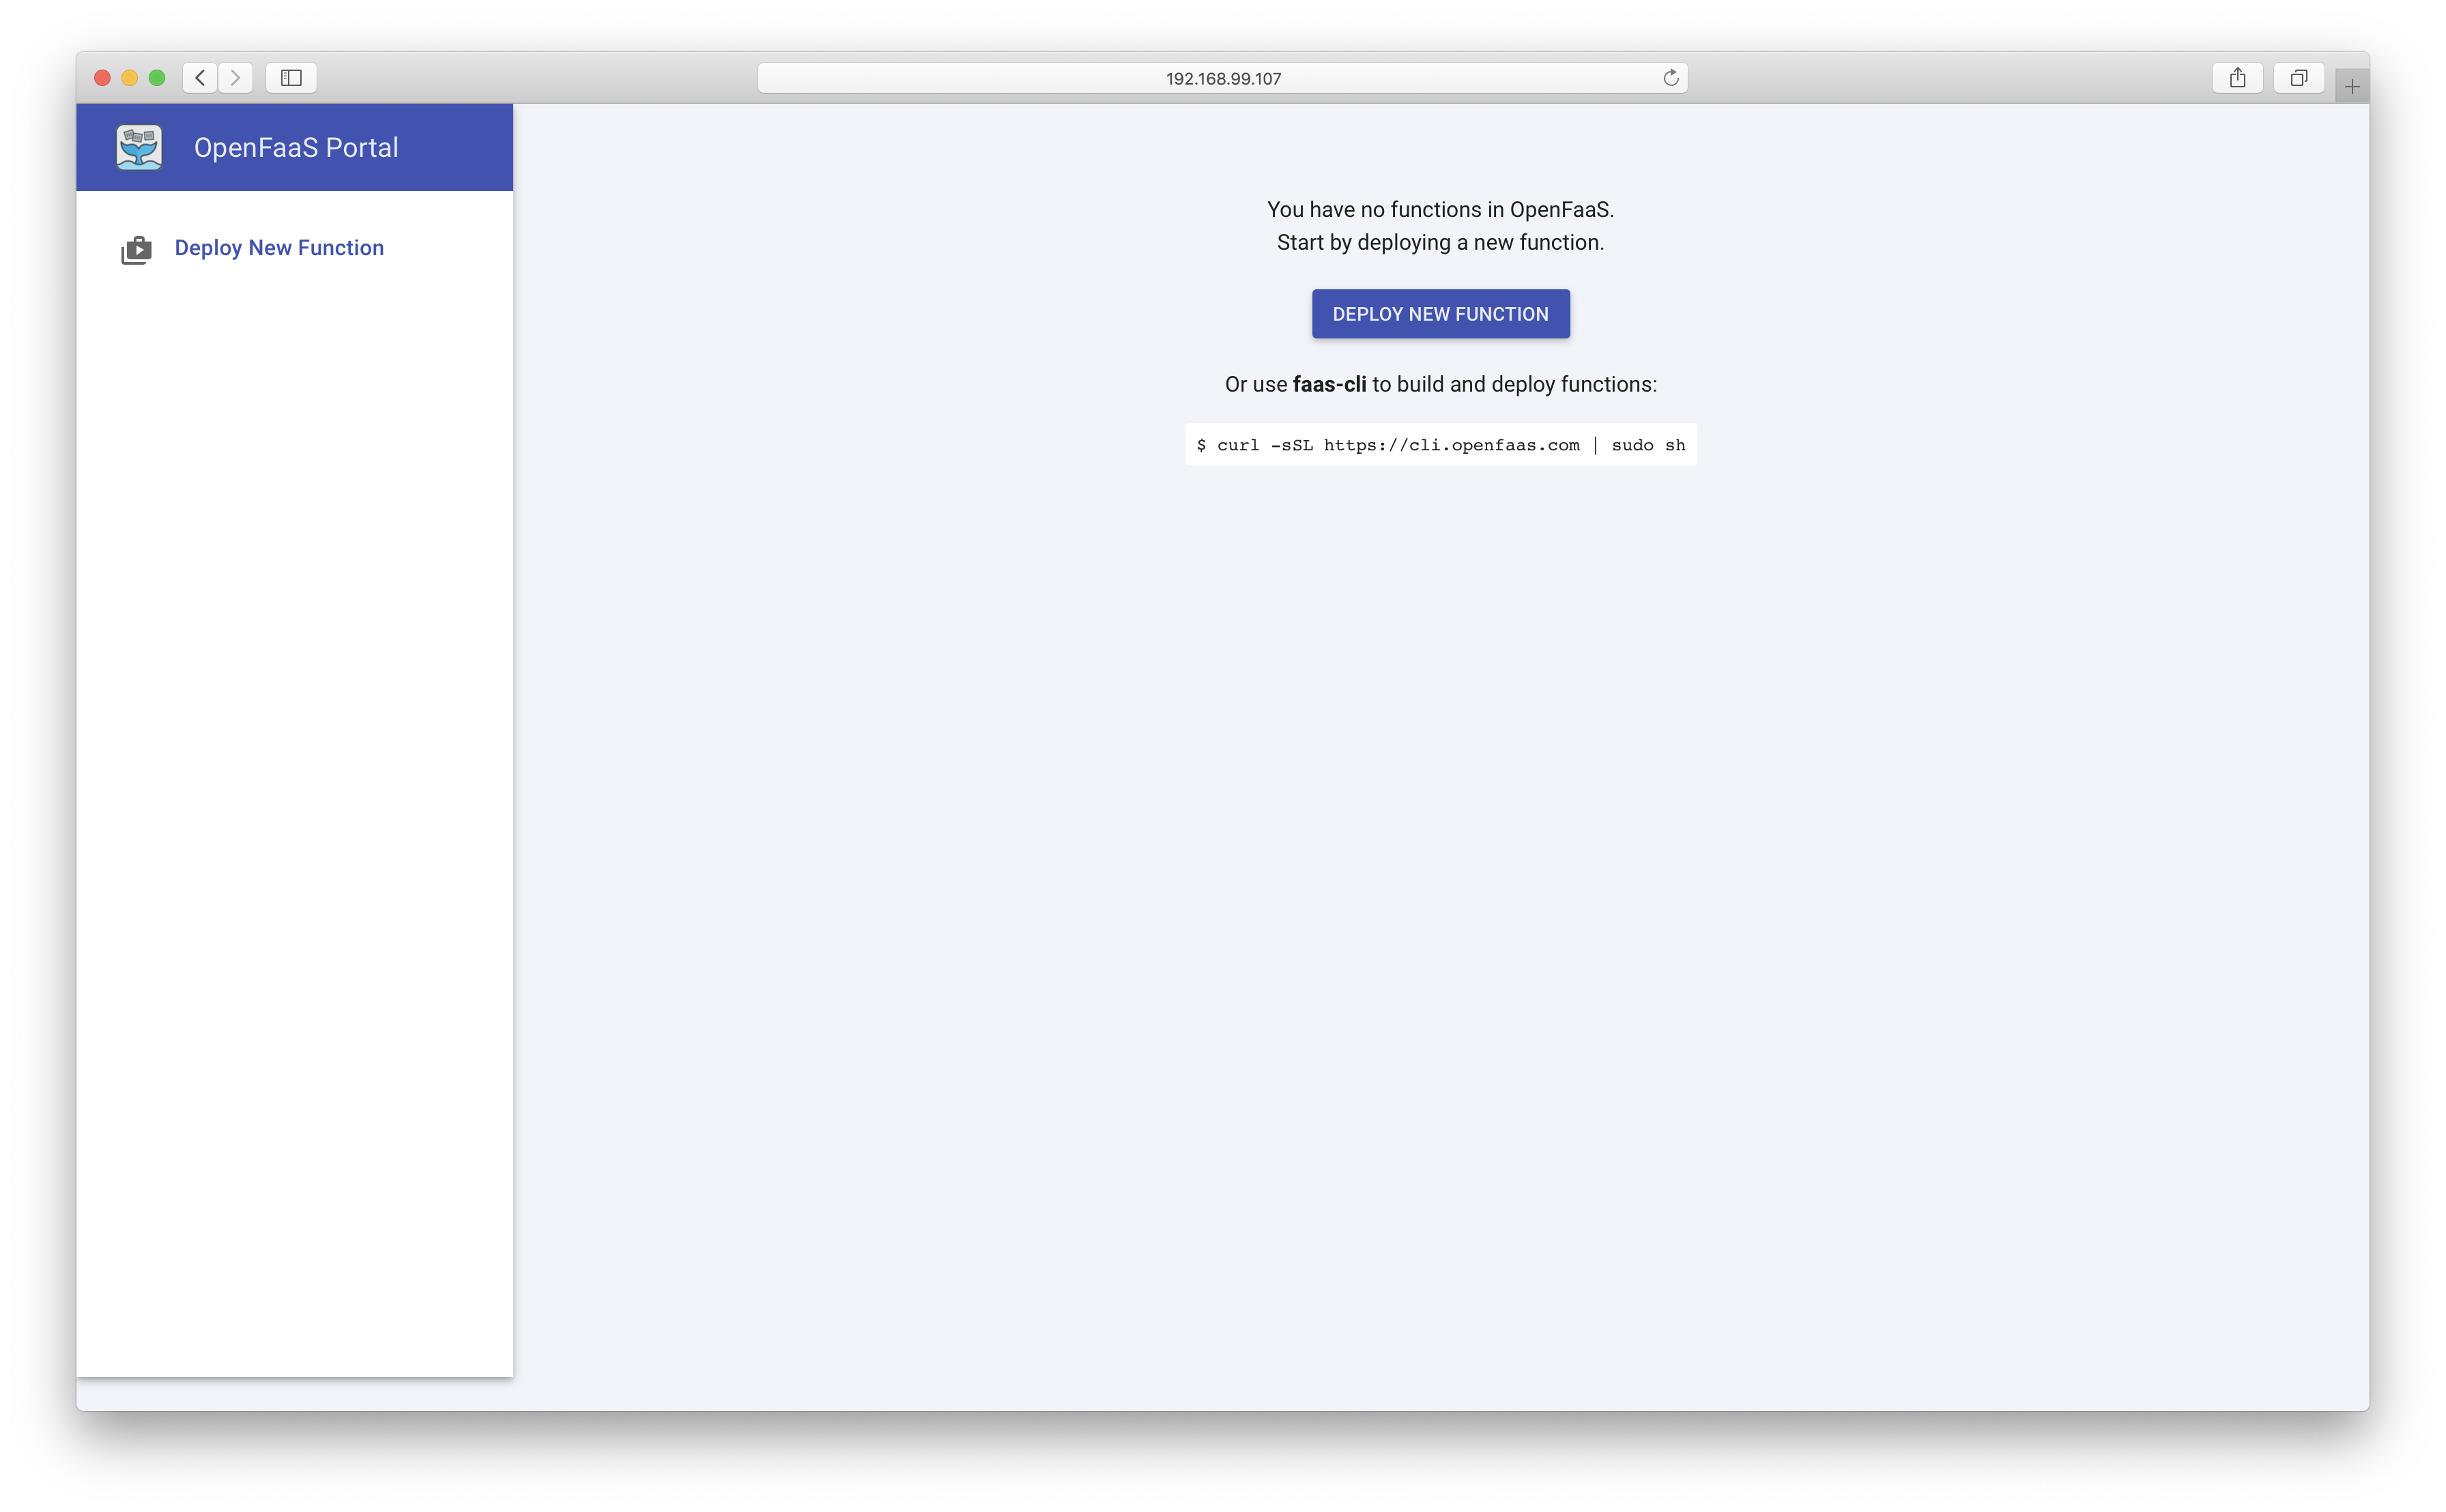
\includegraphics[width=1\textwidth]{img/openfaas-ui.png}
    \caption{OpenFaaS User Interface.}
    \label{fig:openfaas-ui}  
\end{figure}

\subsubsection{Prometheus monitoring}
OpenFaaS voorziet standaard monitoring aan de hand van Prometheus, verschillende metrics kunnen via het Prometheus dashboard worden opgevraagd. Om gebruik te maken van Prometheus moet dit eerst beschikbaar worden gesteld aan de hand van port-forwarding. Om port-forwarding te activeren en het Prometheus te dashboard raadplegen moeten de stappen hieronder ondernomen worden. Gebruikers kunnen  vervolgens interageren met Prometheus via http://localhost:9090. In figuur \ref{fig:openfaas-prometheus} is het dashboard zichtbaar, via deze weg kunnen queries worden uitgevoerd om metrics op te vragen.
\begin{lstlisting}[language=bash]
# Configureer port-forwarding.
$ kubectl port-forward deployment/prometheus 9090:9090 -n openfaas
\end{lstlisting}

\begin{figure}
    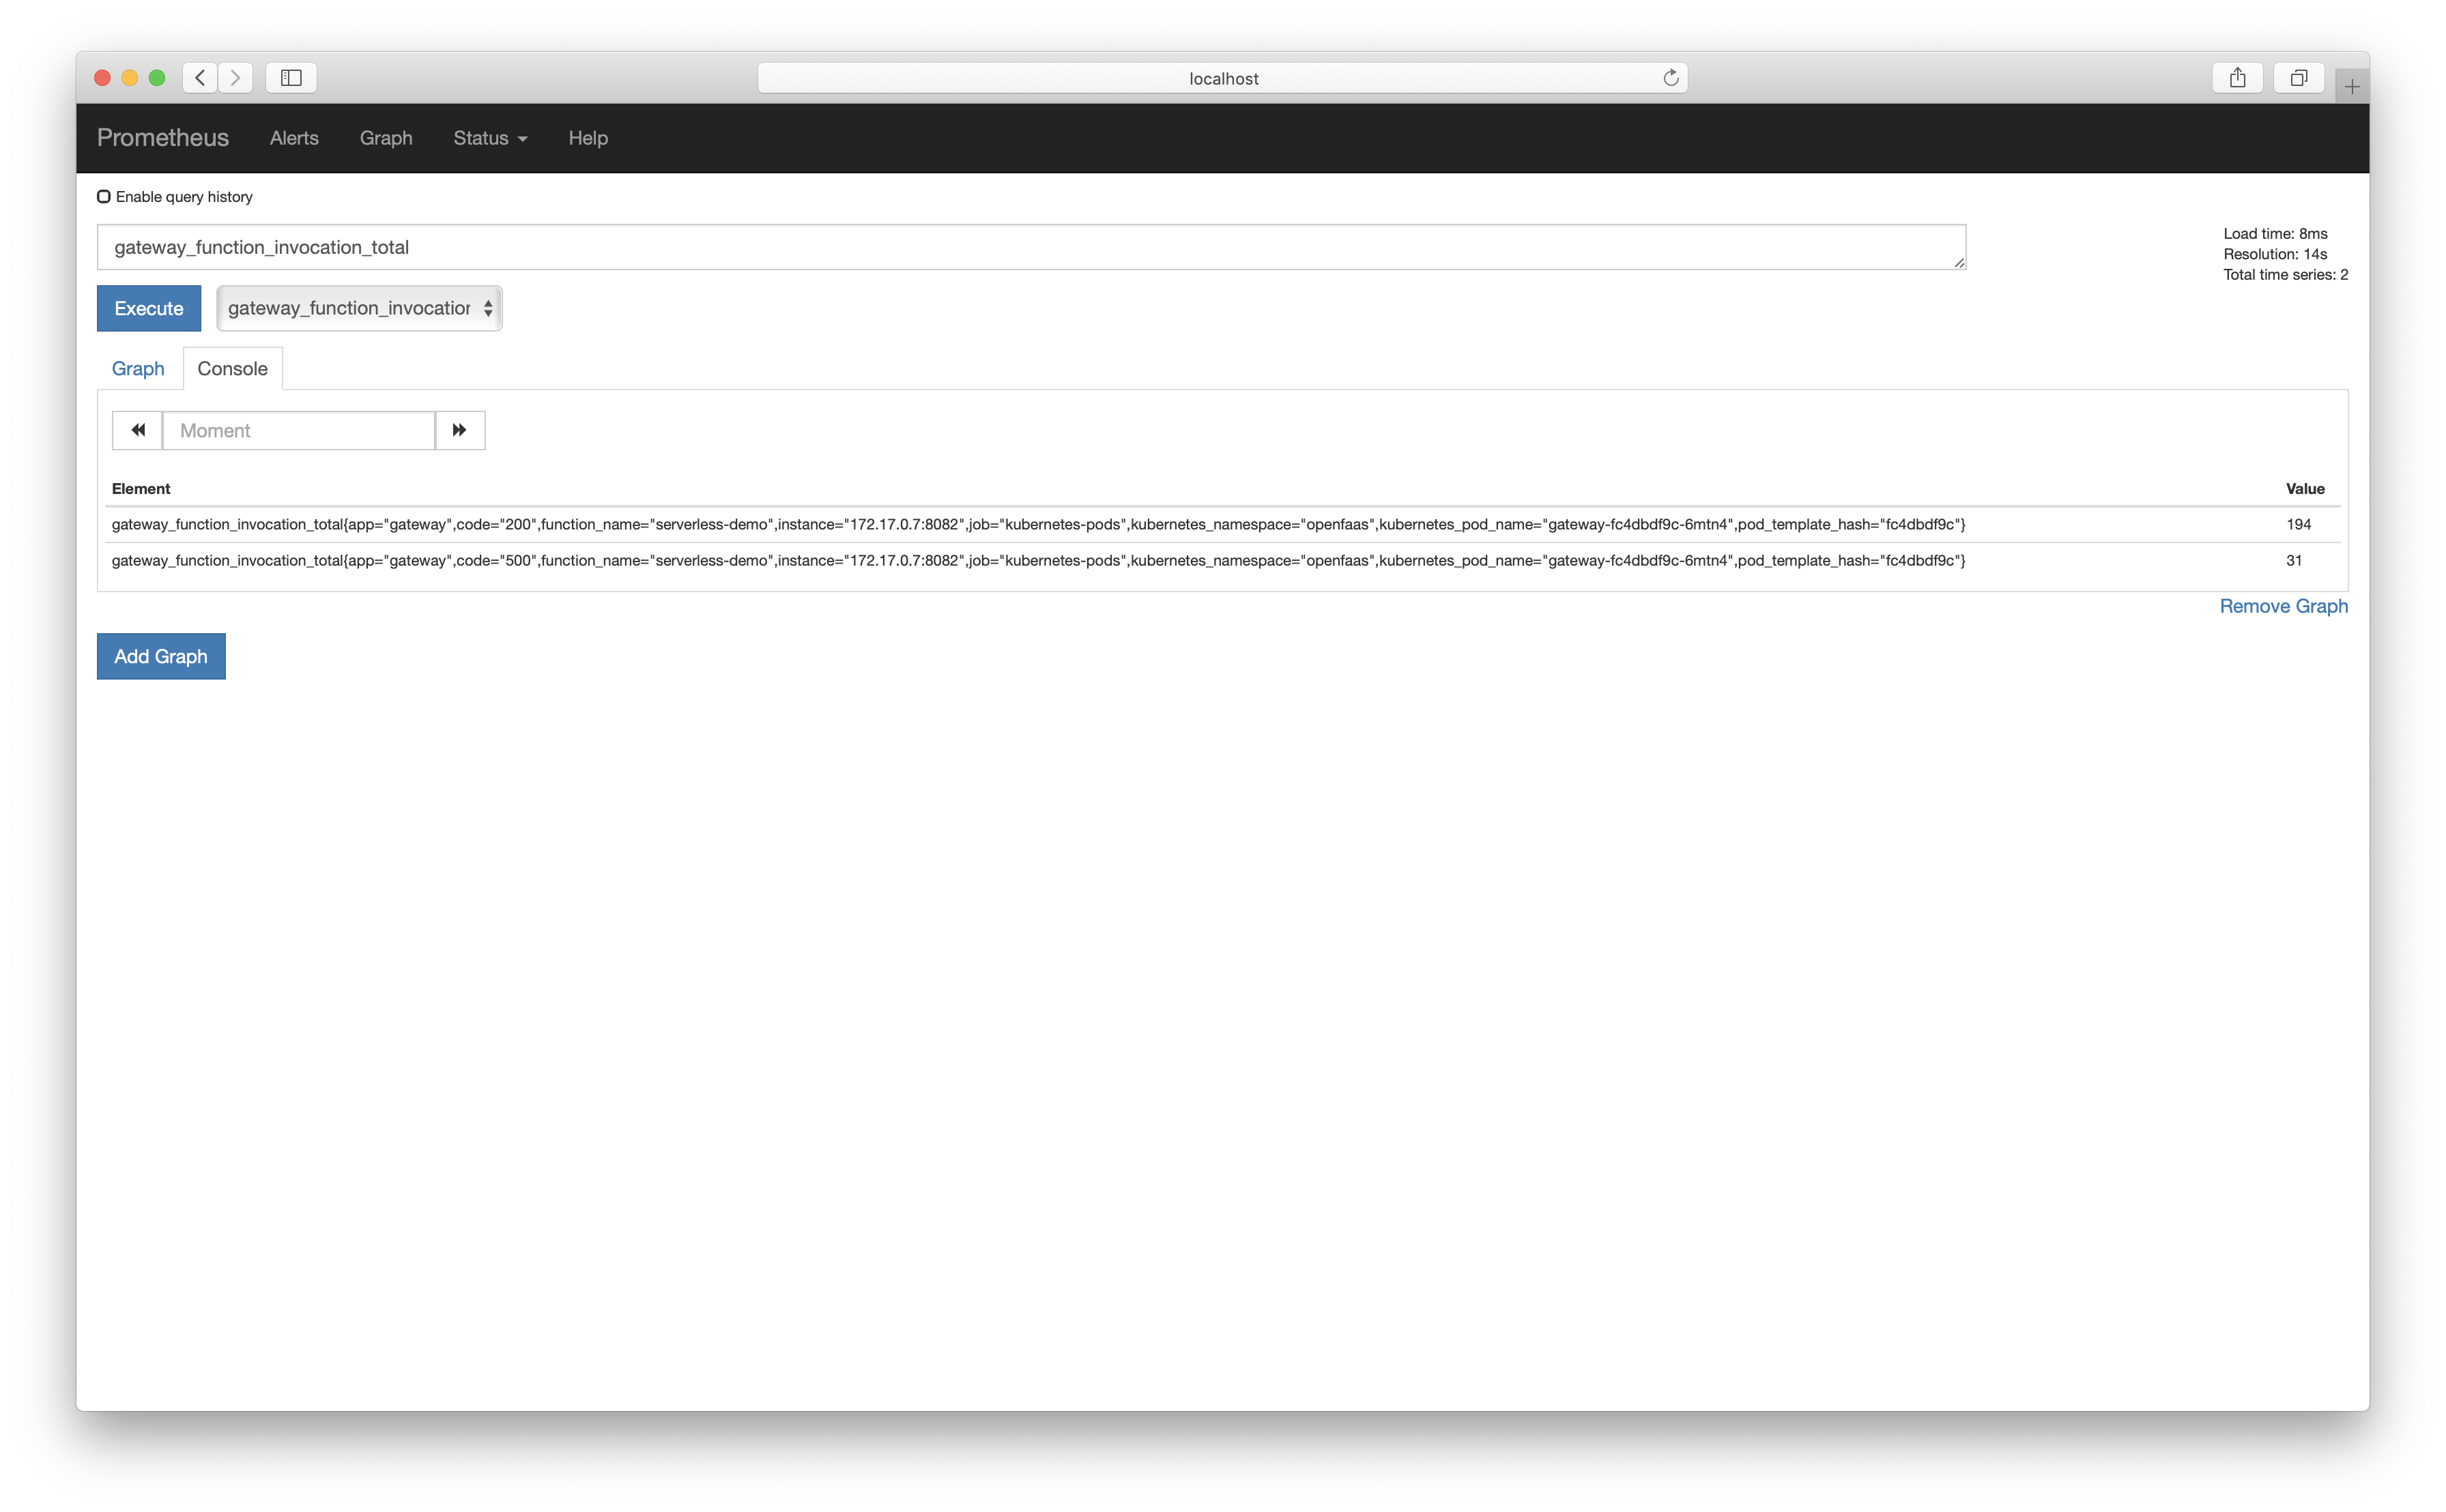
\includegraphics[width=1\textwidth]{img/openfaas-prometheus}
    \caption{OpenFaaS Prometheus dashboard.}
    \label{fig:openfaas-prometheus}  
\end{figure}

\subsection{Schaalbaarheid OpenFaaS}
Een van de requirements waaraan het framework moet voldoen is automatische schaalbaarheid. Wanneer het aantal pods van de functie wordt opgevraagd dan is er te zien dat er initieel maar één draait, zie figuur \ref{fig:openfaas-scalability-1}.
\begin{figure}
    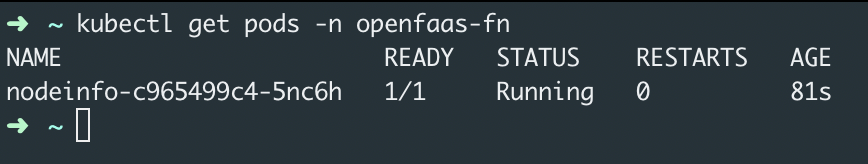
\includegraphics[width=1\textwidth]{img/openfaas-scalability-1.png}
    \caption{OpenFaaS standaard pods.}
    \label{fig:openfaas-scalability-1}  
\end{figure}

Wanneer de functie zeer veel wordt aangeroepen met bijvoorbeeld loop statements, m.a.w. indien de HTTP load verhoogt, dan zullen we zien dat wanneer we de pods opnieuw opvragen deze opschalen zonder dat hier iets moet voor worden gedaan. In figuur \ref{fig:openfaas-scalability-2} is te zien hoe de functie wordt aangeroepen en hoe de pods automatisch schalen. De functie die dit demonstreert is een eenvoudige functie\footnote{https://bit.ly/2HGg85y} die informatie over de node ophaalt en deze teruggeeft aan de gebruiker, dit is een community functie die beschikbaar is in de OpenFaaS store en via de UI kan worden gedeployed. Hoe meer requests de functie moet verwerken, hoe meer pods er worden opgebracht. Als de requests worden gestopt dan schaalt OpenFaaS weer down zoals in figuur \ref{fig:openfaas-scalability-3} te zien is. Standaard zal er steeds een container blijven draaien, dit zorgt ervoor dat cold-starts worden vermeden. Er worden dus steeds een klein aantal resources verbruikt maar dit is een bewuste keuze omdat de container ervoor zorgt dat hoge latency wordt vermeden. In OpenFaaS kan de gebruiker zelf bepalen wanneer en hoe de functie moet geschaald worden, zo kan er ook gekozen worden om een container volledig af te zetten als deze voor een bepaalde tijd geen requests ontvangt.

\begin{figure}
    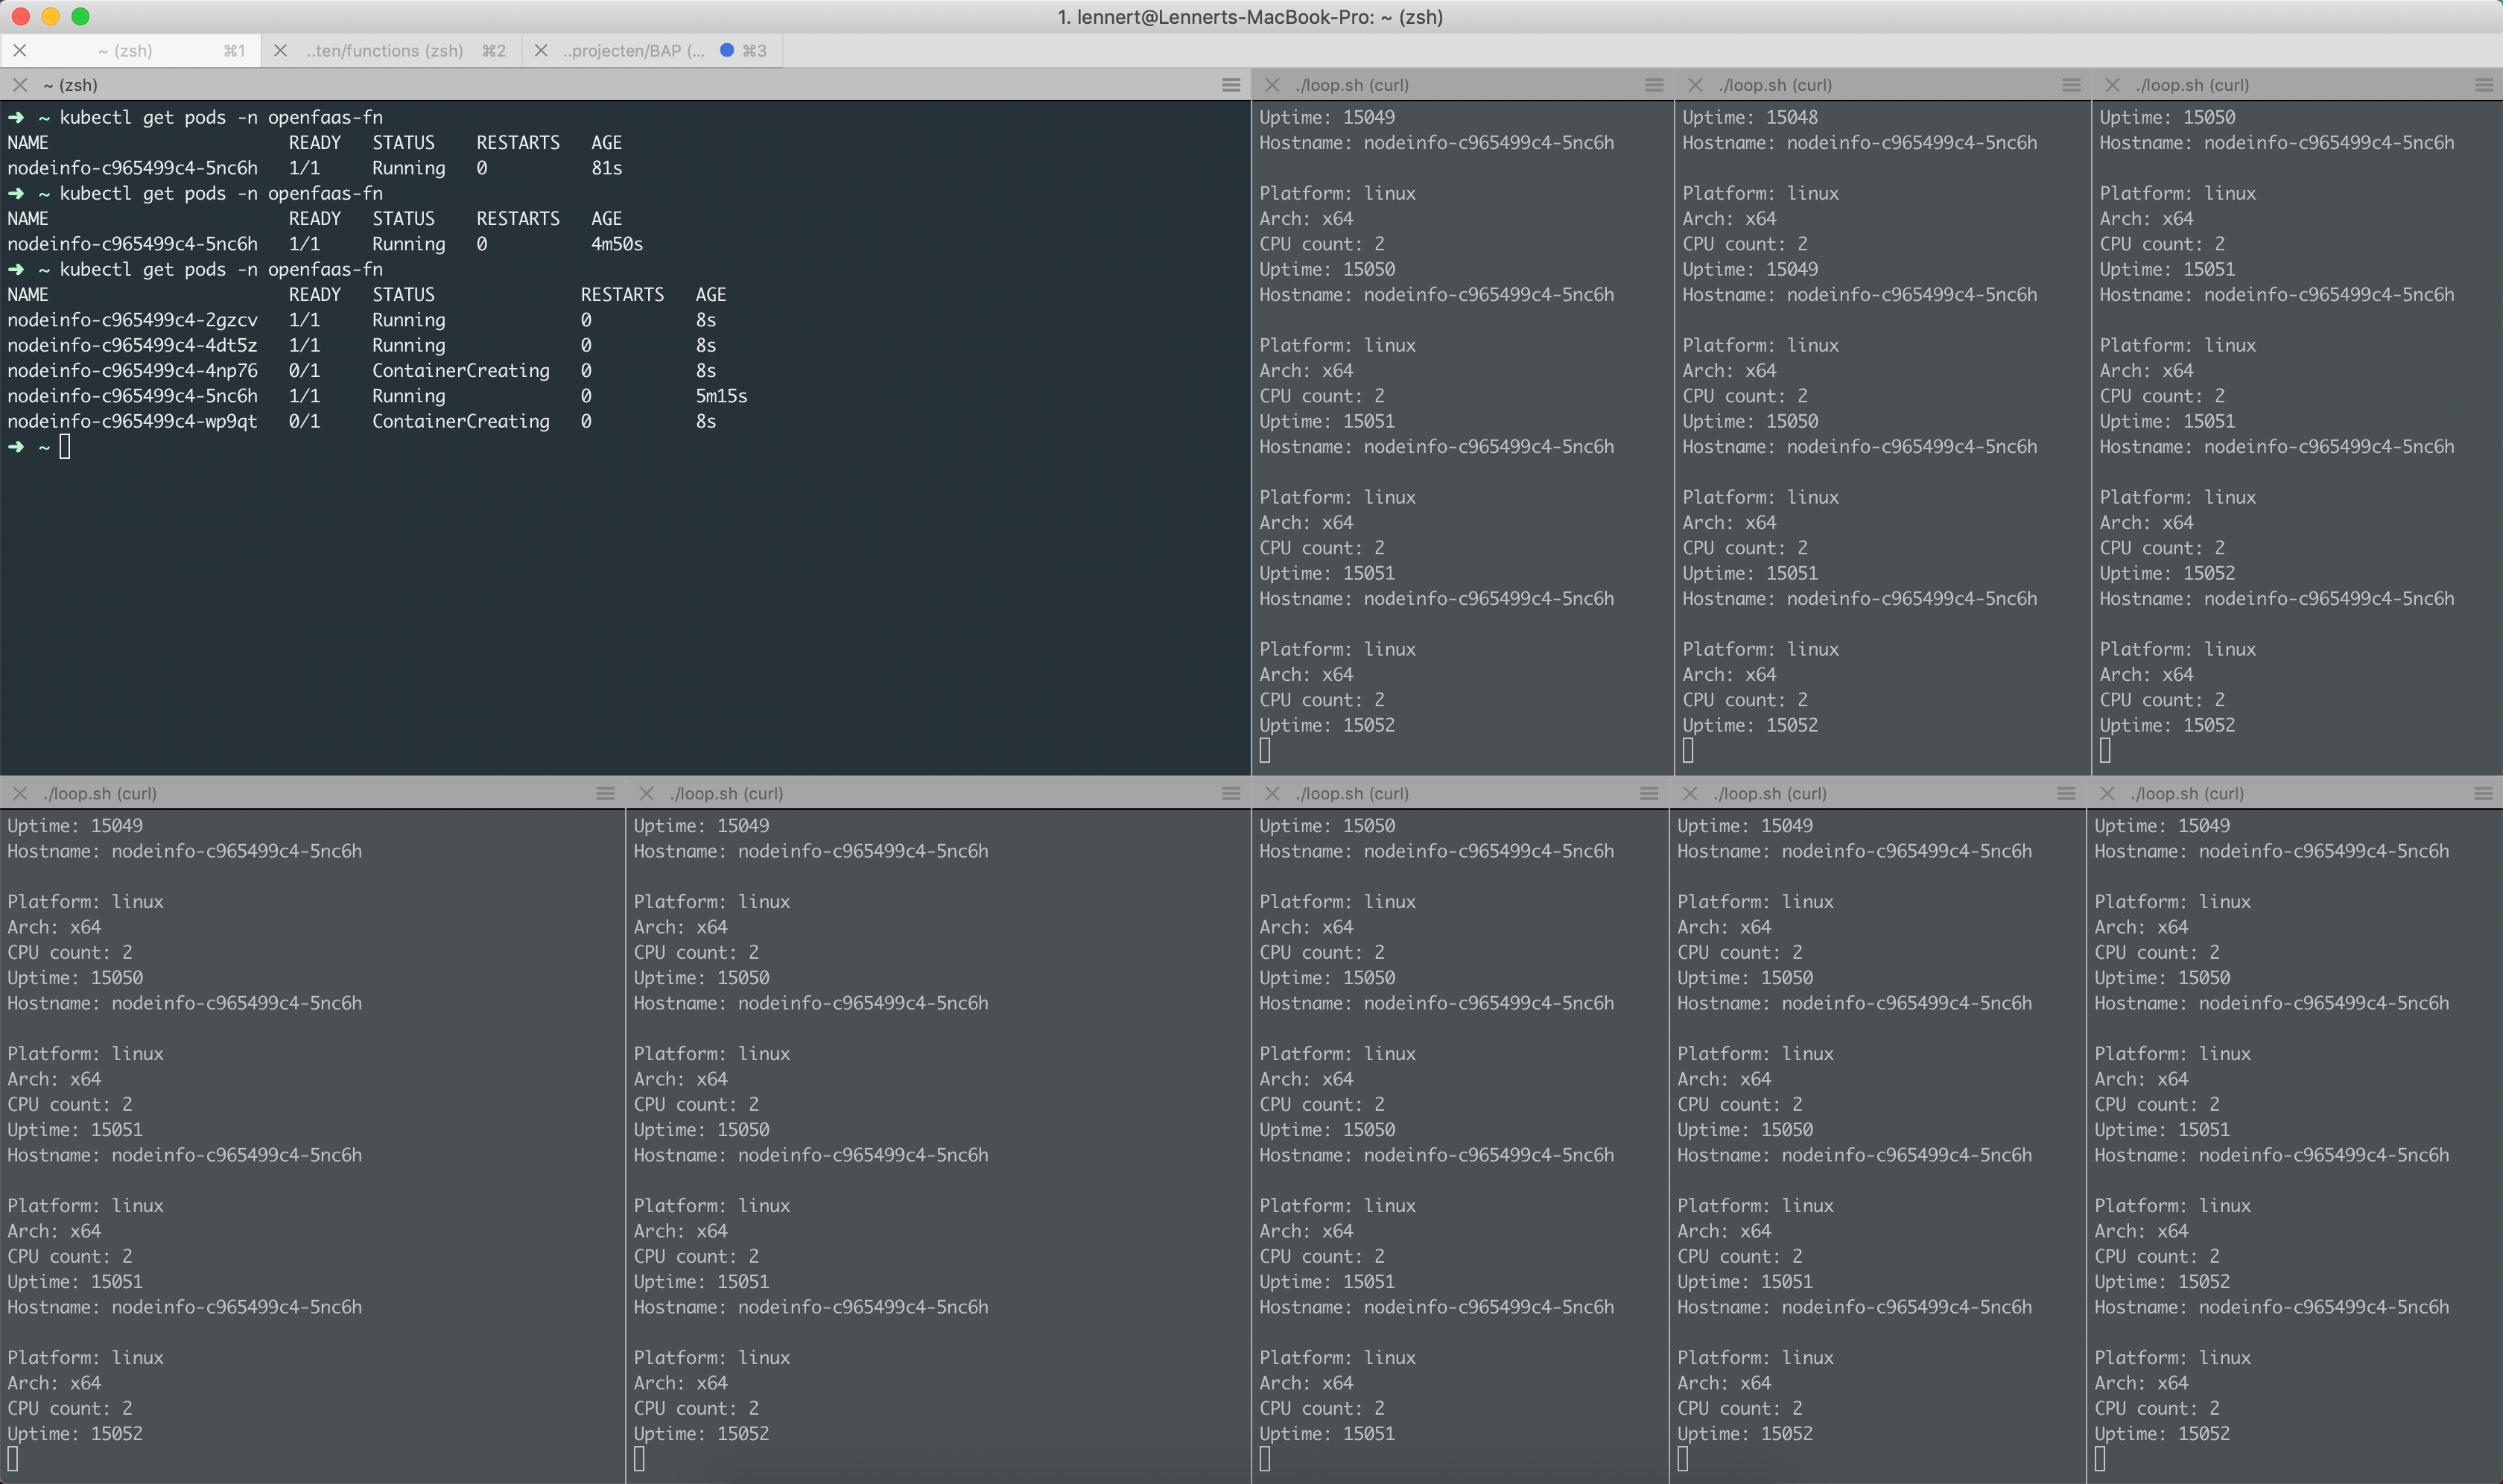
\includegraphics[width=1\textwidth]{img/openfaas-scalability-2.png}
    \caption{OpenFaaS pods schalen up na HTTP GET requests.}
    \label{fig:openfaas-scalability-2}  
\end{figure}

\begin{figure}
    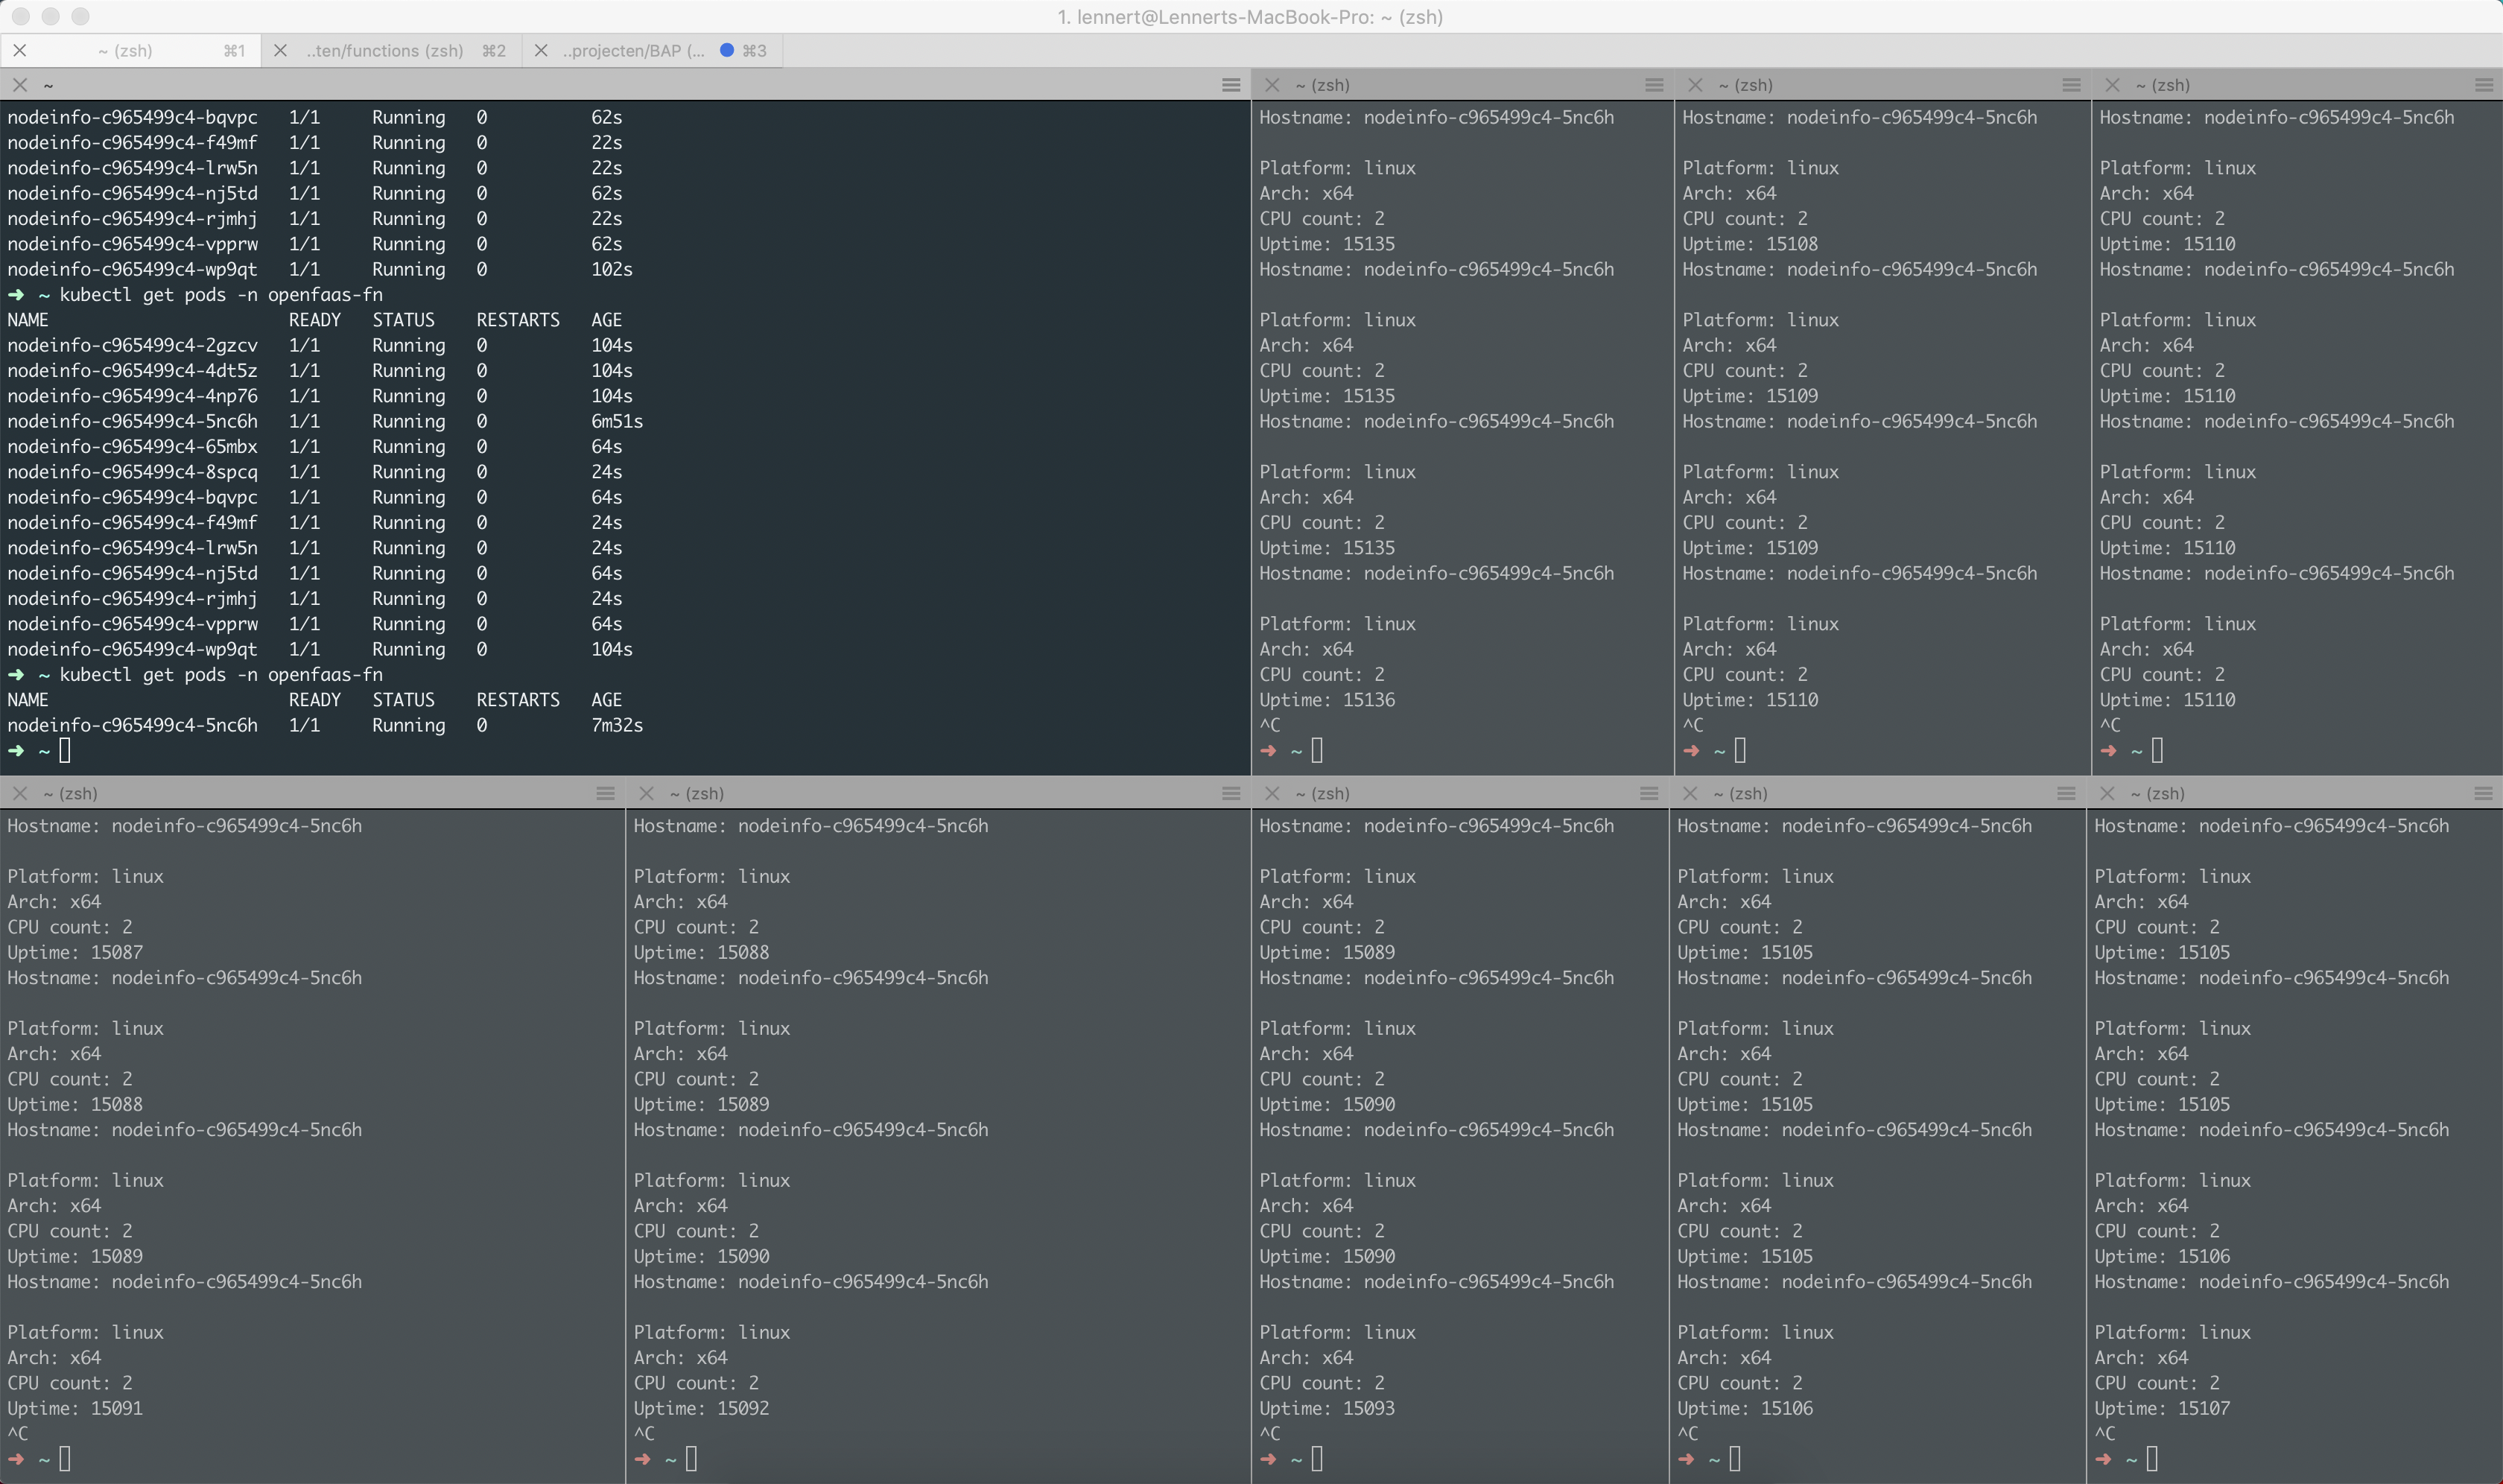
\includegraphics[width=1\textwidth]{img/openfaas-scalability-3.png}
    \caption{OpenFaaS pods schalen down wanneer requests worden afgebroken.}
    \label{fig:openfaas-scalability-3}  
\end{figure}

\subsection{Verzamelen functie data}
Om de frameworks met elkaar te vergelijken wordt de uitvoeringstijd van de geschreven Python functie onder de loep genomen. De tijd die nodig is voor het uitvoeren van de functie, vanaf dat de HTTP request wordt verzonden t.e.m. het moment dat er een response volgt en de functie eindigt, wordt weggeschreven naar een csv bestand. Het csv bestand zal in een later stadium van dit onderzoek gebruikt worden om enkele operaties op uit te voeren die inzicht geven in de uitvoeringstijd van de functie. De demofunctie wordt tweehonderd keer aangeroepen via een HTTP request dat de string ''Test'' wegschrijft naar een Google spreadsheet bestand. Na afloop van wordt de uitvoeringstijd weggeschreven naar het bestand uitvoeringstijd-openfaas.csv dat terug te vinden is in bijlage \ref{sec:uitvoeringstijd-demofunctie}. Onderstaande code voorziet de loop waarmee de functie wordt aangeroepen en de uitvoeringstijd wordt weggeschreven. 

\begin{lstlisting}[language=bash]
$ cat openfaas-loop.sh
#!/bin/bash
touch uitvoeringstijd-openfaas.csv
echo Uitvoeringstijd OpenFaaS >> uitvoeringstijd-openfaas.csv
for i in {1..200};
do
    curl -s -w "%{time_total}\n" -d "Test" -X GET -o /dev/null
    $OPENFAAS_URL/function/serverless-demo  \
    >> uitvoeringstijd-openfaas.csv
done

# Voer uit vanuit zelfde shell als installatie, deze kent de 
# omgevings variabelen.
$ OPENFAAS_URL=$OPENFAAS_URL ./openfaas-loop.sh
\end{lstlisting}

Omdat de Python functie gebruikmaakt van de Google API en per request moet authenticeren, wordt ook de uitvoeringstijd van een eenvoudige ''Hello World'' functie, geschreven in Python, gemeten en weggeschreven naar een csv bestand met de naam uitvoeringstijd-openfaas-hello.csv. Beide frameworks zullen dus ook getest worden via een functie die enkel afhankelijk is van het framework zelf. De functie die hiervoor geschreven werd is terug te vinden in bijlage \ref{sec:openfaas-hello-world-functie}. De Python ''Hello World'' functie kan op een gelijkaardige manier als de andere demofunctie worden gedeployed. De bijhorende loop die de data wegschrijft naar een bestand is ook in de bijlage terug te vinden. De weggeschreven data is toegevoegd in bijlage \ref{sec:uitvoeringstijd-hello-world}. Analoog aan de Python demofunctie wordt de tijd vanaf dat het request wordt verstuurd tot de tijd dat er een response wordt ontvangen gemeten in seconden.

\newpage
\section{Fission}
Het tweede framework dat onder de loep wordt genomen is Fission. Nubera gaf bij de start van dit onderzoek aan dat zij reeds geëxperimenteerd hadden met Fission en hier enige interesse voor hebben opgebouwd. Aan het eind van dit onderzoek moet het duidelijk zijn waarin beide frameworks verschillen en welk het meest interessant zou kunnen zijn volgens de opgestelde requirements.

\subsection{Installatie Fission}
Fission kan worden geïnstalleerd bovenop de Minikube cluster die eerder werd geïnstalleerd. De Fission installatie werd geautomatiseerd in een shell script en is terug te vinden in bijlage \ref{sec:installatie-fission} onder de naam Installatiescript Fission. De installatie bestaat uit enkele stappen die rechtstreeks uit de documentatie\footnote{https://docs.fission.io/installation/} van Fission komen. Aan het installatiescript werden eveneens additionele stappen toegevoegd voor het opzetten van een Fission UI, indien de gebruiker instemt, dit als vergelijking met de UI die OpenFaaS aanbiedt. Er werd gekozen voor de laatste stabiele versie van Fission, versie 1.2.0.

\begin{lstlisting}
# Clone de repository van dit onderzoek.
$ git clone git@github.com:LennertMertens/BAP.git
$ cd BAP/broncode/installatie
# Indien u enkel Fission wenst te installeren voer dan volgende uit:
$ source fission-install.sh

# Als u alle frameworks wilt installeren op Minikube:
$ source install.sh
\end{lstlisting}

\subsection{Deployment demofunctie}
De werking hoe functies gedeployed worden is verschillend van OpenFaaS en vereist iets meer aandacht van de gebruiker. Initieel was de bedoeling om gebruik te maken van een Kubernetes secret om de credentials voor de Google API in op te slaan. Fission ondersteunt echter niet dezelfde acties als OpenFaaS en de secrets die worden gecreëerd kunnen  niet op de gewenste manier in de functie worden gebruikt. Er wordt geopteerd om daarom te werken met een Docker image\footnote{https://cloud.docker.com/repository/docker/lennertmertens/python-env} die de nodige componenten zoals credentials, voor authenticatie met de Google API, en nodige pip packages bevat. De Docker image is gebaseerd op de standaard environment image die Fission aanbiedt, nl. fission/python-env\footnote{https://hub.docker.com/r/fission/python-env/}.

\subsubsection{1. Aanmaak Docker image}
Het gebruik van een custom Python Docker image stelt gebruikers in staat deze te configureren naar eigen wensen en noden. De image kan worden gepubliceerd in een Docker registry op Docker hub. De onderdelen waaruit deze image is opgebouwd zijn hieronder opgesomd. De Docker image is gebaseerd op bestaande Docker files die werden ontwikkeld door de medewerkers van het Fission project, voor dit onderzoek werden de bestaande bestanden bewerkt, de link naar de code is steeds toegevoegd als voetnoot. De image kan worden gebouwd en worden opgeladen naar een Docker hub (of een andere) repository aan de hand van de commando's in het codeblok.

\begin{itemize}
    \item Dockerfile: in bijlage \ref{sec:dockerfile-fission} is de default Dockerfile\footnote{https://github.com/fission/fission/blob/master/environments/python/Dockerfile-2.7} te vinden die wordt voorzien in het Fission framework. Fission voorziet een aantal standaard images specifiek voor een aantal programmeertalen, deze images bevatten dependencies voor het uitvoeren van functies geschreven in een specifieke taal.
    \item Requirements.txt: Dit bestand bevat verschillende packages die met pip worden geïnstalleerd in de image. Standaard zijn er een aantal voorzien in de default Fission image. Er werden nog enkele extra packages toegevoegd voor het uitvoeren van de functie die zelf geschreven werd. Het bestand is terug te vinden in bijlage \ref{sec:requirements-fission}.
    \item Server.py\footnote{https://github.com/fission/fission/blob/master/environments/python/server.py}: Het Python script dat gekopieerd wordt naar de Docker image is een script dat werd geschreven door de medewerkers van het Fission project en zorgt ervoor dat functies die gebruik maken van deze image serverless kunnen worden aangeroepen. 
    \item Credentials.json: De Docker image bevat eveneens de credentials die werden aangemaakt voor gebruik van de Google API, deze zijn privé en voor elke gebruiker verschillend. Het credentials bestand dient in dezelfde map als de Dockerfile te worden geplaats zodat functies hiervan later gebruik kunnen van maken. 
\end{itemize}

\begin{lstlisting}[language=bash]
# Build de docker image vanuit de directory met de Dockerfile.
$ cd custom-docker-image
$ ls -l
total 40
-rw-r--r--  1 lennert  staff   257B May  6 18:03 Dockerfile
-rw-r--r--  1 lennert  staff   2.3K May  6 20:42 credentials.json
-rw-r--r--  1 lennert  staff   131B May  6 20:43 requirements.txt
-rw-r--r--  1 lennert  staff   4.0K May  6 17:34 server.py

# lennertmertens is de naam van de Docker Hub repository.
$ docker build -t lennertmertens/python-env . 
$ docker push lennertmertens/python-env
\end{lstlisting}

\subsubsection{2. Deploy functie}
Er is een verschil in werking in deployment van functies tussen Fission en OpenFaaS, Fission vereist een aantal additionele stappen die hieronder in detail worden doorlopen. Het is van belang dat alle pods die Fission aanmaakt beschikbaar zijn alvorens volgende stappen uit te voeren. Het duurt ongeveer een tweetal minuten, na installatie, tot alle pods beschikbaar zijn voor deployment van functies.
\\\\
Fission werkt by-default op een andere manier dan OpenFaaS. Wanneer een functie wordt gedeployed via OpenFaaS, dan zal het framework steeds één container met de functie laten draaien, dit zorgt ervoor dat cold-starts niet kunnen voorkomen. Fission daarentegen zet containers die niet in gebruik zijn onmiddellijk af waardoor bij het aanroepen van functies cold-starts kunnen voorkomen en latency optreedt. Om beide frameworks op een gelijkwaardige manier te beoordelen wordt de instelling aangepast zodanig dat Fission ook steeds een container met de functie heeft draaien zodat cold-starts worden vermeden en de gegevens later met elkaar vergelijkbaar zijn. Om hetzelfde gedrag als bij OpenFaaS na te bootsen, wordt er gebruik gemaakt van een Newdeploy executor zoals eerder besproken werd in sectie \ref{sec:fission-executors}. Volgende stappen maken het mogelijk om de Python demofunctie te deployen en beschikbaar te stellen via een URL langs de Fission router.

\begin{lstlisting}[language=bash]
# 1. Maak een environment aan waarin de Python functie zal 
# worden uitgevoerd, de environment wordt opgesteld met 
# de eerder gemaakte Docker image.
$ fission environment create --name python-env \
--image lennertmertens/python-env

# 2. Deploy de geschreven Python functie (cd in de 
# directory met de Python code).
# Stel eveneens in dat er minimum een pod draait met de functie.
$ fission function create --name serverless-demo \
--code handler.py --env python-env \
--minscale 1 --executortype newdeploy

# 3. Voeg een pad toe voor toegang via de Fission router.
$ fission route create --function serverless-demo \
--url /serverless-demo
\end{lstlisting}
 
\subsubsection{handler.py}
Handler.py is het Python script dat geschreven werd in sectie \ref{sec:demofunctie} en werd aangepast specifiek voor Fission. De manier waarop functies in Fission worden aangeroepen is verschillend van OpenFaaS. De functies hebben een main methode nodig om uitvoerbaar te zijn, daarom dat de aanpassingen werden aangebracht. De Fission functie maakt eveneens gebruik van credentials die aanwezig zijn in de Docker container. Het Python script dat wordt gedeployed op het Fission framework is terug te vinden in bijlage \ref{sec:demofunctie-fission}.

\subsection{Uitvoeren demofunctie}
De demofunctie reageert op HTTP GET requests, deze actie kan worden getriggered op verschillende manieren. Fission voorziet in de command line tools een commando voor het testen van functies die gedeployed werden op het framework. De output van het test commando weergeeft logs en kan gebruikt worden voor het troubleshooten van functies. Tijdens het deployen van de demofunctie werd er eveneens een pad voor de functie gedefinieerd, via de Fission router en het aangemaakte pad kan de functie ook worden aangeroepen. Gebruikers kunnen naar het IP adres van de router surfen gevolgd door het pad of kunnen aan de hand van een curl commando de functie opvragen.

\begin{lstlisting}[language=bash]
# Aanroep functie met test commando.
$ fission function test --name demo-functie
# Aanroep functie met curl.
$ curl -X GET $FISSION_ROUTER/serverless-demo
$ curl -X GET -d `Test string` $FISSION_ROUTER/serverless-demo
\end{lstlisting}

\subsection{Gebruik Fission}
\subsubsection{User Interface}
De installatie voorziet standaard geen meegeleverde user interface. Achteraf kan een UI worden geïnstalleerd maar deze blijkt echter niet te voldoen aan de verwachtingen. De GitHub repository\footnote{https://github.com/fission/fission-ui} waarvan de UI werd gedownload geeft eveneens aan dat deze zeker niet production ready is en momenteel nog een early alpha versie is. Het installatiescript exporteert een variabele met de link voor toegang tot de UI. De standaardpoort waarop de UI draait is poort 31319. In figuur \ref{fig:fission-ui} is te zien hoe de UI eruitziet. Wanneer de UI wordt, geopend wordt er echter een foutboodschap weergegeven die luidt als volgt: ''Fission server supports API v2 only -- v1 is not supported. Please upgrade your Fission client/CLI''. Functies en environments die worden toegevoegd aan Fission worden niet weergegeven in de UI, het is ook niet mogelijk via de UI nieuwe componenten te definiëren. De UI werkt niet en dit is een known-issue op GitHub.
\begin{figure}
    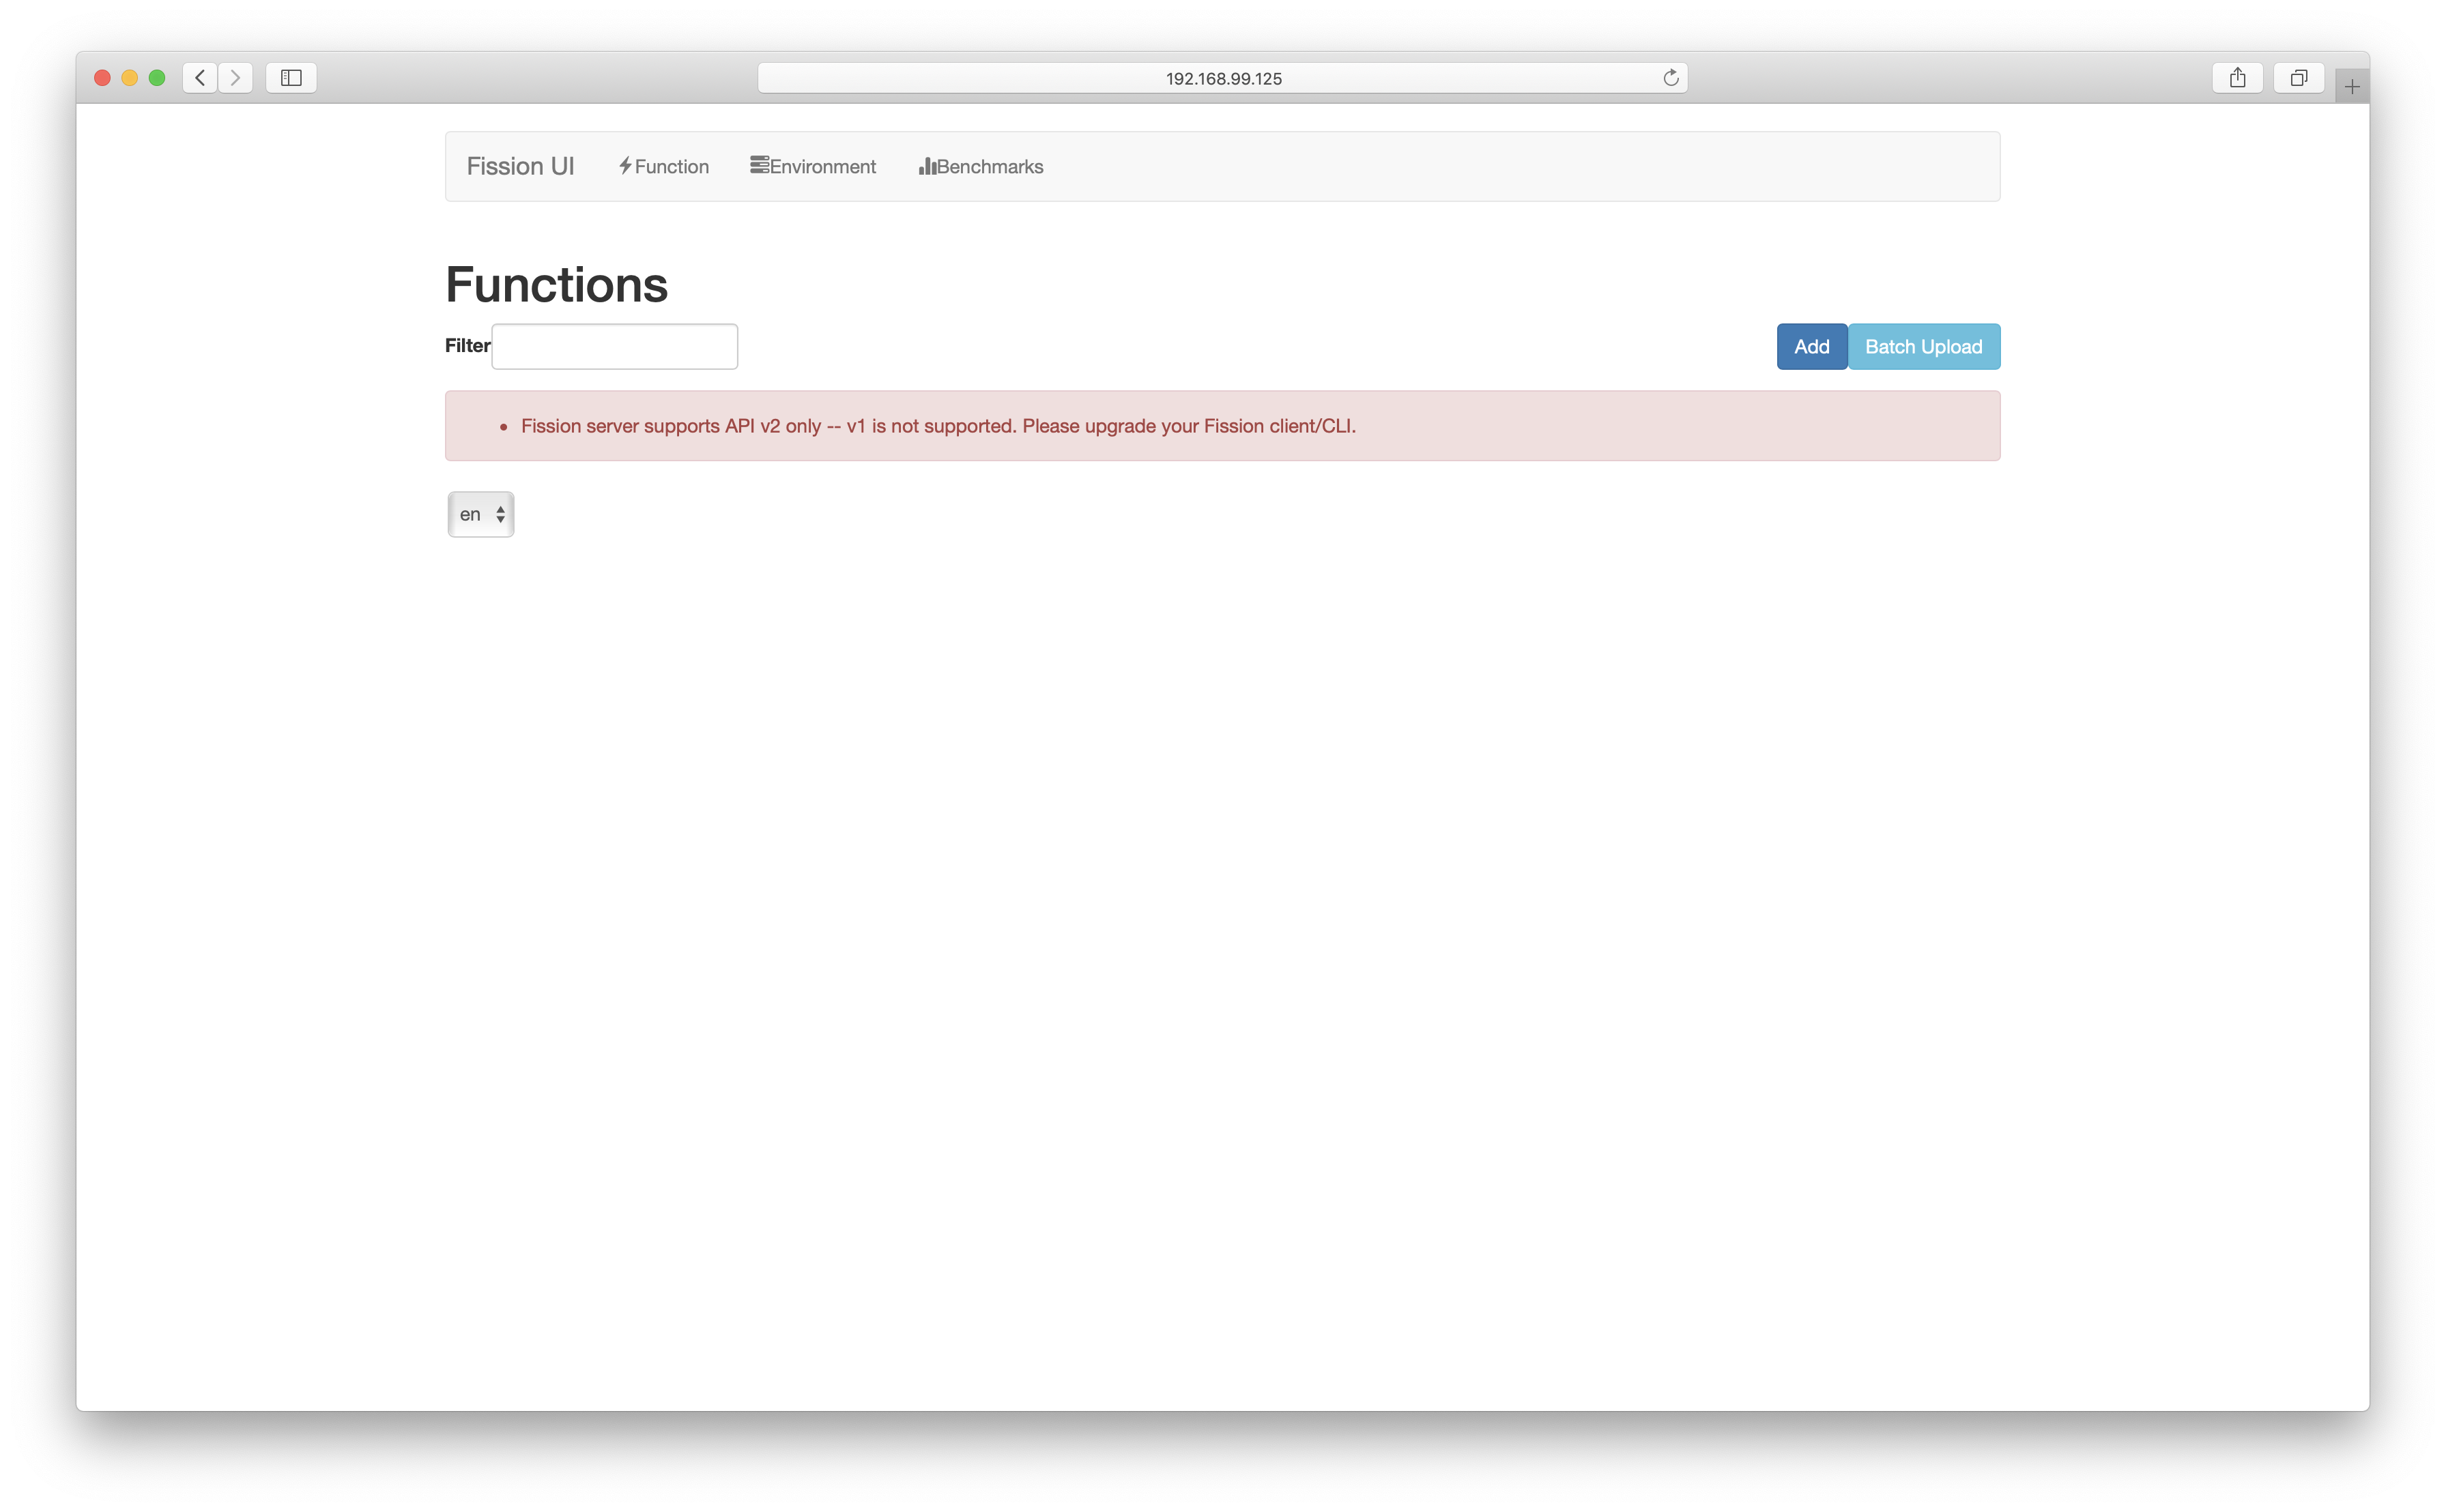
\includegraphics[width=1\textwidth]{img/fission-ui.png}
    \caption{Fission User Interface met foutmelding.}
    \label{fig:fission-ui}  
\end{figure}

\subsubsection{Command line tools}
Fission voorziet net zoals OpenFaaS command line tools voor het beheer van het framework. Via de CLI kunnen functies worden gedefinieerd, routes en environments gecreëerd, en triggers geconfigureerd. Alle taken en opdrachten worden uitgevoerd via de CLI. De CLI tools zijn eenvoudig in gebruik en in de documentatie worden goede voorbeelden voorzien om hiermee aan de slag te gaan. De werking van de CLI en de handelingen in Fission werden bestudeerd aan de hand van een boek over serverless frameworks geschreven door \textcite{McKendrick2018}.

\subsubsection{Prometheus monitoring}
Prometheus wordt standaard voorzien in de installatie van Fission. Wanneer port forwarding wordt geactiveerd kunnen er queries worden verstuurd om metrics op te vragen via een webinterface. De code die de client voor querying activeert, is hieronder beschreven, nadien kan de data worden opgevraagd via http://localhost:9090. Het is handig om via deze client verschillende queries uit te voeren om inzicht te krijgen in functies en hun performantie. Achteraf kunnen er additionele dashboards die gebruik maken van Prometheus metrics worden geïnstalleerd. Zo is het achteraf mogelijk Grafana of een ander dashboard voor monitoring te installeren bovenop Istio (Dit wordt standaard met Fission meegeleverd). De verschillende mogelijke monitoringsdashboard worden niet in dit onderzoek besproken.

\begin{lstlisting}[language=bash]
# Expose de Prometheus client via http://localhost:9090.
$ kubectl -n fission port-forward  \ 
  $(kubectl -n fission get pod -l app=prometheus,\
  component=server -o name) 9090
\end{lstlisting}

\subsection{Schaalbaarheid Fission}
Om de schaalbaarheid van Fission te demonstreren wordt er gebruik gemaakt van een demofunctie die terug te vinden is in de Fission repository op GitHub, onder de naam hello.js\footnote{https://github.com/fission/fission/blob/master/examples/nodejs/hello.js}. De demofunctie die hier wordt gebruikt is een simpele ''Hello World'' applicatie geschreven in Node.js. Alvorens er getest kan worden op schaalbaarheid wordt de functie op analoge manier gedeployed als de demofunctie die in Python geschreven werd. Er moet eerst wel een Node.js environment worden aangemaakt en bij het definiëren wordt gekozen voor een minscale van 1 en een Newdeploy executor om automatische schaalbaarheid te voorzien. De stappen om de omgeving klaar te zetten zijn hieronder beschreven. Wanneer de load te zwaar wordt voor één pod om deze te verwerken dan zullen er additionele functie pods worden aangemaakt en wordt er automatisch load balancing tussen de functie pods voorzien.

\begin{lstlisting}[language=bash]
# 1. Aanmaak Node.js environment.
$ fission environment create --name node-env \
--image fission/node-env

# 2. Deploy de hello.js functie.
$ fission function create --name hello \
--code hello.js --env node-env \
--minscale 1 --executortype newdeploy

# 3. Maak een route voor de functie.
$ fission route create --function hello --url /hello
\end{lstlisting}

Om de schaalbaarheid te testen werd vanuit de functie  aangeroepen via een oneindige loop in meer dan 20verschillende Terminal vensters. Echter bleek de functie niet te schalen en werden er geen metrics opgehaald uit de function pods. De metrics zijn nodig om te beslissen of een functie moet op- of neerschalen, in figuur \ref{fig:fission-scalability-issue} is te zien dat ''Target'' unkown is en dus erop wijst dat metrics niet worden opgehaald, desondanks dat Fission op aanbevolen wijze werd geïnstalleerd en Metrics-server werd aangezet op de Minikube cluster.
\begin{figure}
    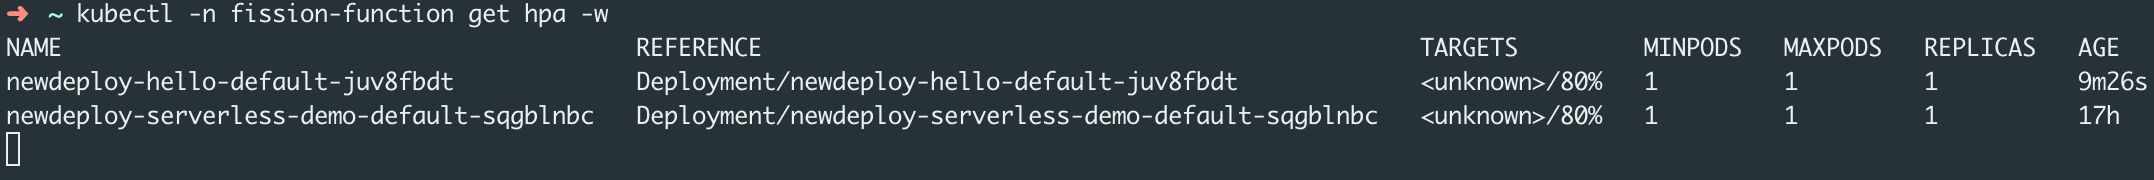
\includegraphics[width=1\textwidth]{img/fission-scalability-issue.png}
    \caption{Fission functie target unknown.}
    \label{fig:fission-scalability-issue}  
\end{figure}

Er werd tot de medewerkers van het Fission project gericht via hun Slack kanaal, hier hebben een aantal medewerkers naar het probleem gekeken maar ook zij konden dit ook niet meteen thuisbrengen. Het is mogelijk dat de issue veroorzaakt wordt door de Minikube setup hoewel autoscaling via OpenFaaS wel lukt en na verder onderzoek ook blijkt dat Metrics-server uit andere pods wel metrics kan ophalen. Bijgevolg werd er een issue aangemaakt in het Fission Github project om de medewerkers formeel op de hoogte te stellen van de problemen waarmee ik te kampen heb gekregen. Het is jammer dat door deze issue de autoscaling niet kon worden gedemonstreerd maar dit is dus wel degelijk beschikbaar in Fission en werkt in normale omstandigheden analoog aan de autoscaling via OpenFaaS. In bijlage \ref{sec:fission-slack-issue} is de communicatie via Slack terug te vinden en bijlage \ref{sec:fission-github-issue} is de bijhorende GitHub issue present, de issue\footnote{https://github.com/fission/fission/issues/1182} werd afgehandeld maar hierop werd ook geen concrete oplossing geboden. Op GitHub werd wel bevestigd dat dit geen probleem is met Fission maar wel met onderliggende componenten. Desondanks de mislukte demonstratie gaan we ervan uit dat Fission autoscaling werkt wanneer beide frameworks tegen elkaar worden afgewogen.

\subsection{Verzamelen functie data}
Zoals eerder beschreven zal er een vergelijking tussen de frameworks worden gemaakt onder andere op basis van uitvoeringstijd van de functie. De tijd die wordt gemeten voor het uitvoeren van de Python demofunctie is diegene vanaf dat de HTTP request wordt verzonden t.e.m. het moment dat er een response volgt en de functie eindigt. De uitvoeringstijd wordt weggeschreven naar een csv bestand dat later zal gebundeld worden tot één bestand dat terug te vinden is in bijlage \ref{sec:uitvoeringstijd-demofunctie}. De metingen voor beide frameworks werden achtereenvolgens uitgevoerd op identiek dezelfde omgeving. Onderstaande code voorziet de loop waarmee de functie wordt aangeroepen en de uitvoeringstijd wordt weggeschreven. De loop wordt net zoals bij het OpenFaaS framework tweehonderd keer aangeroepen.

\begin{lstlisting}[language=bash]
$ cat fission-loop.sh
#!/bin/bash
touch uitvoeringstijd-fission.csv
echo Uitvoeringstijd Fission >> uitvoeringstijd-fission.csv
for i in {1..200};
do
    curl -X GET -s -w "%{time_total}\n" -o /dev/null  \
    -d "Test" $FISSION_ROUTER/serverless-demo  \
    >> uitvoeringstijd-fission.csv
done

# Voer uit vanuit zelfde shell als installatie, deze kent de 
# omgevings variabelen.
$ FISSION_ROUTE=$FISSION_ROUTER ./fission-loop.sh
\end{lstlisting}

De demofunctie maakt gebruik van de Google API en moet deze bij uitvoer steeds authenticeren. Daarom worden beide frameworks ook getest aan de hand van een eenvoudige ''Hello World'' functie, geschreven in Python. De uitvoeringstijd van de functie wordt gemeten (in seconden) en wordt weggeschreven naar een csv bestand met de naam uitvoeringstijd-fission-hello.csv. Beide frameworks zullen dus ook getest worden via een functie die enkel afhankelijk is van het framework zelf. De functie die hiervoor geschreven werd is terug te vinden in bijlage \ref{sec:fission-hello-world-functie}. De Python ''Hello World'' functie kan op een gelijkaardige manier als de andere demofunctie worden gedeployed. De bijhorende loop die de data wegschrijft naar een bestand is eveneens in de bijlage terug te vinden. De weggeschreven data is toegevoegd in bijlage \ref{sec:uitvoeringstijd-hello-world}.

